
%In this section is shown the architecture of the ProLine-RM as well as an description of its components. 
In Figure~\ref{fig:architecture} is depicted the architecture of our infrastructure. As shown in this figure, we devised it on the top of the Eclipse Platform and used both Java and Groovy as programming language. Moreover, we used Eclipse Modeling Framework (EMF)\footnote{http://www.eclipse.org/modeling/emf/} to create the SQL model and to reutilize the UML model. MoDisco is used by the infrastructure since it provides an
\textbf{A}pplication \textbf{P}rogramming \textbf{I}nterface - (API) to easily access the KDM model. 

\begin{figure}[!h]
\centering
  % Requires \usepackage{graphicx}
 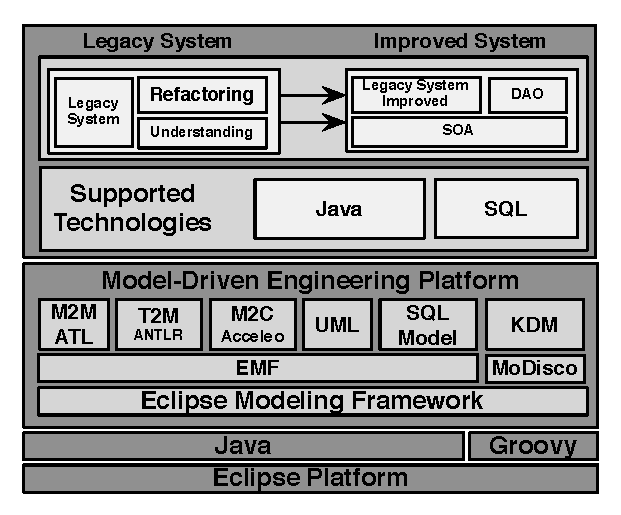
\includegraphics[scale=0.8]{Figuras/Arquitetura_da_Ferramenta}
\caption{Architecture of KnowDIME}
\label{fig:architecture}
\end{figure}



\textbf{A}Nother \textbf{T}ool for \textbf{L}anguage \textbf{R}ecognition -  (ANTLR) is used herein to create parsers to obtain information related to the legacy system's artifacts. Therefore, two parser were developed: (\textit{i}) the first takes as input a Java grammar and generates as output an AST and (\textit{ii}) the second parser is a extension of the first one to identify SQL embedded in the legacy system's source code, i.e., it takes as input a Java source-code and generates as output an AST which contains informations such as, tables, columns, primary keys, etc. Then, to transform these ASTs in PSMs we used an API provided by EMF. Afterwards, all transformation M2M are done by \textbf{A}tlas \textbf{T}ransformation \textbf{L}anguage - ATL, which provides ways to produce a set of target models from a set of source models. Therefore, ATL is used to transform the PSMs to conform the KDM specification and to transform the improved KDM to an UML that represents the target systems. Then, in order to transform this last model in a set of physical artifacts (source code) Acceleo was used, which is based on textual template approach. A template can be thought of as the target text with holes for variable parts. The holes contain metacode which is run at template instantiation time to compute the variable parts. Furthermore, we have used Java Persistence API (JPA) 2.0 to deal with the way relational data is mapped to Java objects. Similarly, RESTful API have been used to implements SOA artifacts.


%Afterwards, all transformation M2M are done by ATL, which is a language...For instance, it is used to transform the PSMs to conform the KDM specification ...into KDM a set of rules were written in ATL, which is a language....., It is used to transform the As-is PIM to a To-be PIM, and finally, to transform this PIM in a PSM conforming the Uml meta model. Then, in order to transform this last model in a set of physical artifacts (source code) Acceleo was used.
 

  %tha  both the source-code of the legacy system and database/SQL queries embedded in into PSM models.


%As can be seen in Figure~\ref{fig:architecture}, all artifacts (source code, feature model, RM and RRM) that the CrossFIRE provides are persisted in a database. These artifacts are persisted in a remote server, available to be reused in the AE phase. This remote server is a physical computer, which is dedicated to run the RESTful API. Therefore, to send these artifacts by the server we have used this API as web service to cache the representation of all artifacts. This server receives requests of the CrossFIRE through RESTful, processes database queries and sends a response to the CrossFIRE by using RESTful as well. Furthermore, we have used Java Persistence API (JPA) 2.0 to deal with the way relational data is mapped to Java objects. To implement the database of the server, the MySQL was chosen.

